\subsection{轴对称和轴对称图形}\label{subsec:czjh1-3-17}

在日常生活里,我们常见到下面一些图形(图 \ref{fig:czjh1-3-60}), 例如,画出的双手,天平的两个称盘等。
如果把它们沿某一条直线翻折过来,其中一个就和另一个重合。

\begin{figure}[htbp]
    \centering
    \begin{minipage}[b]{7cm}
        \centering
        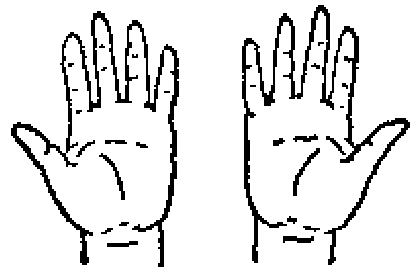
\includegraphics[width=4cm]{../pic/czjh1-ch3-60-a.png}
        \caption*{甲}
    \end{minipage}
    \qquad
    \begin{minipage}[b]{7cm}
        \centering
        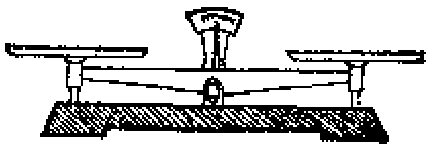
\includegraphics[width=6cm]{../pic/czjh1-ch3-60-b.png}
        \caption*{乙}
    \end{minipage}
    \caption{}\label{fig:czjh1-3-60}
\end{figure}

把一个图形沿着某一条直线折过来,如果它能够与另一个图形重合,
那么我们说这两个图形\zhongdian{关于这条直线对称},
两个图形中的对应点叫做关于这条直线的\zhongdian{对称点},
这条直线叫做\zhongdian{对称轴}。
例如,在图 \ref{fig:czjh1-3-61} 中,$\triangle ABC$ 和 $\triangle A'B'C'$ 关于直线 $MN$ 对称,
点 $A$ 和 $A'$, $B$ 和 $B'$, $C$ 和 $C'$ 是关于直线 $MN$ 的对称点,
直线 $MN$ 是对称轴。

因为两个关于某直线对称的图形是可以互相重合的,所以它们一定全等。

下面,我们研究关于轴对称的两个图形的性质。

根据定义,如果点 $A$ 和 $A'$ 是关于直线 $MN$ 的对称点(图 \ref{fig:czjh1-3-61}),
那么沿 $MN$ 折过来,点 $A$ 与 $A'$ 重合,于是
\begin{align*}
    & AP = PA' \douhao \\
    & \angle MPA = \angle MPA' = Rt \angle \douhao
\end{align*}
也就是直线 $MN$ 垂直平分线段 $AA'$。 因此可得:

\begin{xingzhi}[性质1]
    如果两个图形关于某直线对称,那么对应点的连线被对称轴垂直平分。
\end{xingzhi}

在图 \ref{fig:czjh1-3-61} 中, 把两个图形沿对称轴 $MN$ 对折后,直线 $AB$ 和 $A'B'$ 能够重合。
如果直线 $AB$ 与 $MN$ 相交,那么 $A'B'$ 也与 $MN$ 相交于同一点。 因此,又可以得到:

\begin{xingzhi}[性质2]
    两个图形关于某直线对称,如果它们的对应线段或其延长线相交,那么交点在对称轴上。
\end{xingzhi}

性质1 的逆命题:“如果两个图形的对应点连线被同一条直线垂直平分,那么这两个图形关于这条直线对称” 也是成立的。
我们有时用它判定两个图形是否对称。


\begin{figure}[htbp]
    \centering
    \begin{minipage}[b]{5.5cm}
        \centering
        \begin{tikzpicture}
    \tkzDefPoints{0/0/N, 0/4/M}
    \tkzDefPoints{-0.8/0.8/C, -2.0/0.2/B,  -1.3/3/A}
    \tkzDefPointBy[reflection=over M--N](A)  \tkzGetPoint{A'}
    \tkzDefPointBy[reflection=over M--N](B)  \tkzGetPoint{B'}
    \tkzDefPointBy[reflection=over M--N](C)  \tkzGetPoint{C'}
    \tkzInterLL(M,N)(A,A')  \tkzGetPoint{P}
    \tkzDrawSegments(M,N)
    \tkzDrawPolygon(A,B,C)
    \tkzDrawPolygon(A',B',C')
    \tkzDrawSegment[dashed](A,A')
    \tkzMarkRightAngle(A,P,N)
    \tkzLabelPoints[right](M,N)
    \tkzLabelPoints[above](A,A')
    \tkzLabelPoints[left](B,C')
    \tkzLabelPoints[right](C,B')
    \tkzLabelPoints[above right](P)
\end{tikzpicture}


        \caption{}\label{fig:czjh1-3-61}
    \end{minipage}
    \qquad
    \begin{minipage}[b]{4.5cm}
        \centering
        \begin{tikzpicture}
    \tkzDefPoints{0/0/N, 0/4/M}
    \tkzDefPoints{0/3.5/A, -1.5/0.6/B, 0.4/1.6/C}
    \tkzDefPointBy[reflection=over M--N](A)  \tkzGetPoint{A'}
    \tkzDefPointBy[reflection=over M--N](B)  \tkzGetPoint{B'}
    \tkzDefPointBy[reflection=over M--N](C)  \tkzGetPoint{C'}
    \tkzInterLL(M,N)(B,B')  \tkzGetPoint{D}
    \tkzDrawSegments(M,N)
    \tkzDrawPolygon(A,B,C)
    \tkzDrawPolygon(A',B',C')
    \tkzDrawSegment[dashed](B,B')
    \tkzLabelPoints[left](M,N)
    \tkzLabelPoint[right](A){$A (A')$}
    \tkzLabelPoints[left](B,C')
    \tkzLabelPoints[right](C,B')
    \tkzLabelPoints[above left](D)
\end{tikzpicture}


        \caption{}\label{fig:czjh1-3-62}
    \end{minipage}
\end{figure}


\liti 已知 $\triangle ABC$ 和直线 $MN$ (图 \ref{fig:czjh1-3-62})。

求作:$\triangle A'B'C'$, 使 $\triangle A'B'C'$ 与 $\triangle ABC$ 关于 $MN$ 对称。

\zuofa 1. 作 $BD \perp MN$, 垂足 $D$。 延长 $BD$ 到 $B'$, 使 $DB' = BD$, 得到点 $B$ 的对称点 $B'$。

2. 同法作点 $C$ 的对称点 $C'$。

3. 因为点 $A$ 在对称轴 $MN$ 上,所以点 $A$ 的对称点 $A'$ 与 $A$ 重合。

4. 连接 $A'B'$、$B'C'$、$C'A'$。

$\triangle A'B'C'$ 就是所求的三角形。

\liti 如图,在铁路 $a$ 的同侧有两个工厂 $A$、$B$,要在路边建一个货场 $C$,
使 $A$、$B$ 两厂到货场 $C$ 的距离的和最小。在图上作出点 $C$。

已知;直线 $a$ 和 $a$ 的同侧两点 $A$、$B$(图 \ref{fig:czjh1-3-63})。

求作:点 $C$, 使 $C$ 在直线 $a$ 上,并且 $AC + CB$ 最小。

\zuofa 1. 作点 $A$ 关于直线 $a$ 的对称点 $A'$。

2. 连结 $A'B$ 交 $a$ 于点 $C$。

点 $C$ 就是所求的点。

\zhengming 在直线 $a$ 上另取一点连结 $C'$,连结 $AC$、$AC'$、$A'C'$、$C'B$。

因为直线 $a$ 是点 $A$、$A'$ 的对称轴,点 $C$ 在对称轴上,

$\therefore$ \quad $AC = A'C$, $AC' = A'C'$,

$\therefore$ \quad $AC + CB = A'C + CB = A'B$。

在 $\triangle A'C'B$ 中,

$\because$ \quad $A'B < A'C' + C'B$。

$\therefore$ \quad $AC + CB < AC' + C'B$,

即 \quad $AC + CB$ 最小。

\begin{figure}[htbp]
    \centering
    \begin{minipage}[b]{4.5cm}
        \centering
        \begin{tikzpicture}
    \tkzDefPoints{0/0/M, 4/0/N}
    \tkzDefPoints{0.4/0.8/A, 3.5/1.5/B}
    \tkzDefPointBy[reflection=over M--N](A)  \tkzGetPoint{A'}
    \tkzInterLL(M,N)(A',B)  \tkzGetPoint{C}
    \tkzDefShiftPoint[C](1,0){C'}

    \tkzDrawSegments(M,N  A',B)
    \tkzDrawSegments[dashed](A,A'  A,C  A,C'  A',C'  B,C')
    \tkzLabelSegment[below, pos=0.9](M,N){$a$}
    \tkzLabelPoints[above](A,B)
    \tkzLabelPoints[below](A', C')
    \tkzLabelPoints[below,yshift=0.2em](C)
\end{tikzpicture}


        \caption{}\label{fig:czjh1-3-63}
    \end{minipage}
    \qquad
    \begin{minipage}[b]{9.5cm}
        \centering
        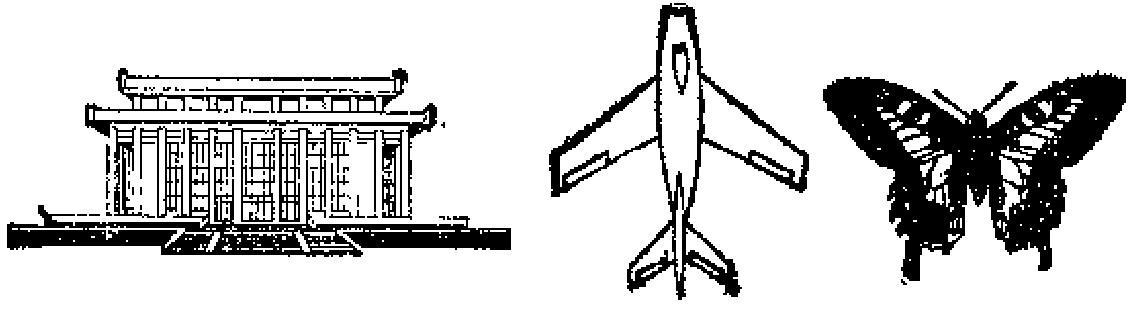
\includegraphics[width=9cm]{../pic/czjh1-ch3-64.png}
        \caption{}\label{fig:czjh1-3-64}
        \end{minipage}
\end{figure}

如果一个图形沿一条直线对折,直线两旁的部分能够互相重合,也就是图形和它本身重合,
那么这个图形叫做\zhongdian{轴对称图形}, 这条直线就是它的对称轴。
例如,等腰三角形是一个轴对称图形,它的底边的垂直平分线是它的对称轴;
角也是轴对称图形,对称轴是角的平分线所在的直线;
线段也是轴对称图形,对称轴是它的垂直平分线。
日常生活中见到的轴对称图形也很多,如图 \ref{fig:czjh1-3-64} 中的图形,都是轴对称图形。

\begin{lianxi}

\xiaoti{如果 $\triangle ABC \quandeng \triangle A'B'C'$, 能否说 $\triangle ABC$ 和 $\triangle A'B'C'$ 是对称的?为什么?}

\xiaoti{已知 $\triangle ABC$。 以边 $BC$ 所在的直线为对称轴, 作一个三角形和它对称。}

\xiaoti{为什么等边三形是轴对称图形? 画出它的对称轴。 共有几条对称轴?}

\end{lianxi}

